% Auto-converted from Optimizing_Gestural_Efficiency.docx via pandoc
% Source section: Background
\chapter{Background}\label{background}

This research views global languages as having
\emph{\textbf{\uline{lexemes}}} (words or phrases) made up of
\emph{\textbf{\uline{lexons}}} (individual unicode characters). For
example, the English lexeme /father-in-law/ has lexons
{[}~f,a,t,h,e,r,-,i,n,l,w~{]}, and the Chinese lexeme \textbf{/岳父/}
(/yuèfù/, /father-in-law/), has lexons {[}~\textbf{岳}, \textbf{父}~{]}.

When using a qwerty keyboard to input English lexemes, the gestural
efficiency is one \emph{\textbf{\uline{lexon}}} (letter) for one
\emph{\textbf{\uline{gesture}}} or 100\%.

Specialty \emph{\textbf{\uline{input methods}}}
(\emph{\textbf{\uline{IME}}}s) enable qwerty keyboards to input
non-English lexons and lexemes. Figure 1 is an example of a Chinese IME.

\begin{figure}[htbp]
\centering
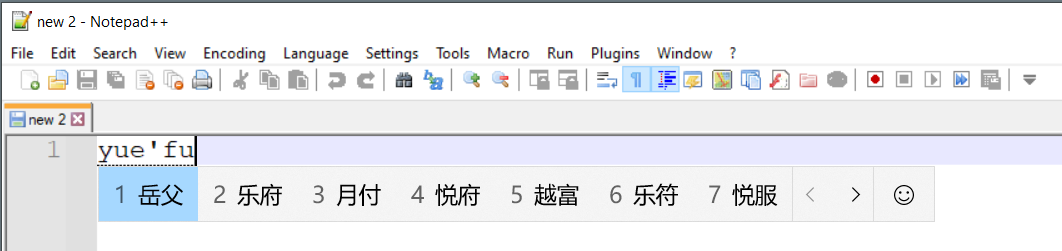
\includegraphics[width=6.5in,height=1.53611in]{media/media/image1.png}
\caption{Chinese Input Method}
\label{fig:auto:1}
\end{figure}


In general, non-English IMEs have gestural efficiencies below 100\%. For
example, The Chinese IME inputs the two lexons with 6-8 qwerty gestures,
for a \emph{\textbf{\uline{gestural efficiency}}}
(\emph{\textbf{\uline{GE}}}) of 25\% - 33\%.

Global language IMEs are software that have dynamic displays indicating
\textbf{\uline{gesture/choice associations}}
(\emph{\textbf{\uline{GCA}}}s). For example

(gestures for choices that lead to lexical input. Factors that
contribute to increased IME usability are:

\begin{itemize}
\item
  Gestural Efficiency- Minimize the number of gestures required to
  effect lexical input.
\item
  Touch typing -- Minimize time and mental effort to learn
  gestures+choices GCA without reference to the display.
\item
  Visual Scan -Minimize time and visual effort to locate displayed
  gesture+choice
\end{itemize}

The goal of this research is to produce IMEs which increase efficiency
for global language by reducing the number of gestures needed to input
lexemes and lexons.

The current research pulls from several diverse fields, including
computer science, linguistics, and human factors psychology. This
background section introduces concepts and terms to facilitate
presentation of the research.

\section{Non-QWERTY Lexica}\label{non-qwerty-lexica}
In linguistics, a collection of words and multi-word set phrases is a
\emph{\textbf{lexicon}} (pl: \emph{\textbf{lexica}}) (Masini, 2019).
Individual items in a \emph{\textbf{\uline{lexicon}}} are
\emph{\textbf{\uline{lexemes}}}.

This research defines \emph{\textbf{lexica}} as \textbf{\uline{sets}} of
statistically common lexon sequences for populations of (computer)
users. So, the English language lexicon contains lexemes /a/, /the/, /in
front of/, and /father-in-law/. Note that, for this research, lexica are
for written, not spoken, language. Figure 2 shows examples of lexica are
their user communities.

\begin{longtable}[]{@{}
  >{\raggedright\arraybackslash}p{(\columnwidth - 2\tabcolsep) * \real{0.6122}}
  >{\raggedright\arraybackslash}p{(\columnwidth - 2\tabcolsep) * \real{0.3878}}@{}}
\toprule
\begin{minipage}[b]{\linewidth}\raggedright
Lexicon
\end{minipage} & \begin{minipage}[b]{\linewidth}\raggedright
User Community
\end{minipage} \\
\midrule
\endhead
English Phrases & English Speakers \\
Chinese Phrases & Chinese Speakers \\
American English Legal Terms & American Lawyers \\
Emoticons & Texters \\
\bottomrule
\end{longtable}

Figure Examples of Lexica and
Associated User Communities

Lexemes are \emph{\textbf{\uline{sequences}}} of the 149,186 characters
available in the Unicode standard (\emph{Unicode FAQ}, 2023). In
addition to the \emph{\textbf{Basic Latin}} characters on the qwerty
keyboard, Unicode contains many types of Unicode characters including
emojis, numbers, diacritics, technical symbols, musical symbols,
International Phonetic Alphabet (IPA) and Braille. It also contains
language specific symbols in \emph{\textbf{scripts}}, such as Arabic,
Greek, Hebrew, Japanese (Hiragana, Katakana), and Chinese.

\section{Lexons are from the Unicode
Standard}\label{lexons-are-from-the-unicode-standard}

Unicode is effectively a superset of all inputtable characters (Allen et
al., 2012b). Many linguistic input sets are indicated in Figure 3, taken
from (Allen et al., 2012b). The typologies (Alphabets Abjads, Abugidas,
Logosyllabaries, Simple Syllabaries, Featural Syllabaries) are useful in
understanding the relationships between a language's lexemes and its
lexons.

\begin{figure}[htbp]
\centering
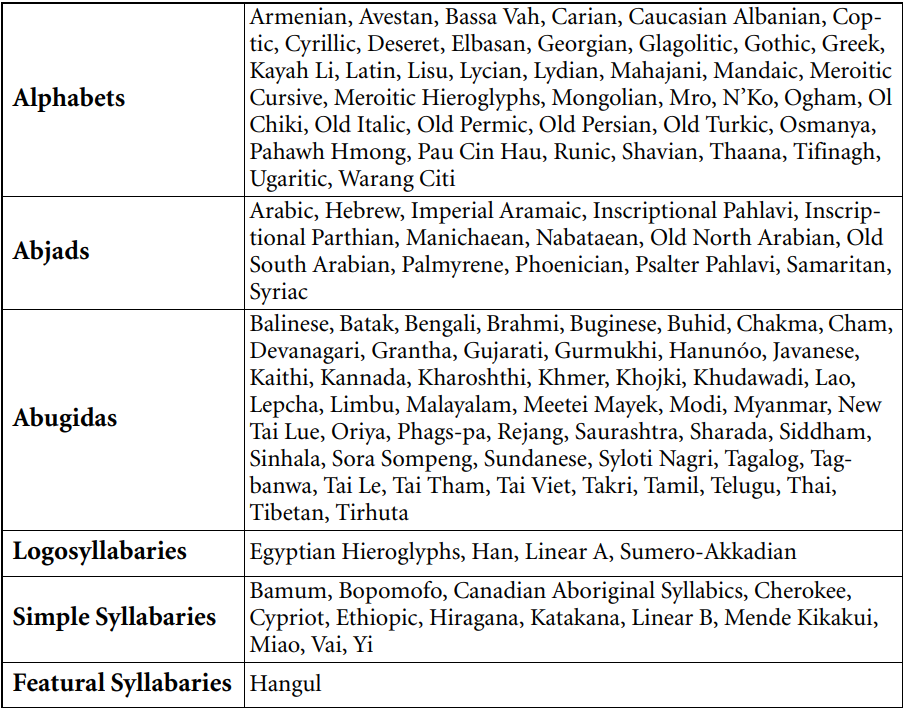
\includegraphics[width=2.70427in,height=2.12037in]{media/media/image2.png}
\caption{Unicode Standard Script Typology}
\label{fig:auto:2}
\end{figure}


\section{Lexical Input Strategies}\label{lexical-input-strategies}
There are two different strategies for software to give users choices
leading to lexical input:

\begin{itemize}
\item
  Character selection: Users choose individual characters comprising
  lexical items one at a time. An example is keyboarding English.
\item
  Sequenced selection: Users make choices from a display associating
  gestures on peripherals with lexemes. Examples are methods used in
  mobile phone texting apps to select lexemes instead of letters. More
  complex examples present sequences in which individual selections
  cause subsequent choices to be presented; so, a sequence of selections
  lead to input lexical items.
\end{itemize}

Although symbol selection systems use more gestures (e.g., keystrokes)
for input, they have the advantage of being able to select any lexical
item by its comprising symbols. Sequenced selection input systems, on
the other hand, reduce gesture counts for many lexemes; but, given the
productive nature of language, cannot encompass entire lexica.

Given the certainty that sequenced selection systems will not include
all lexemes, they must be supplemented with symbol selection systems.
So, \textbf{\emph{µ}Lex} apps are either character selection systems or
combined character \textbf{+} sequence selection systems.

\section{Lexical Input Peripheral
Devices}\label{lexical-input-peripheral-devices}

\emph{\textbf{µLex}} is device-agnostic; it can be used with common
input peripherals keyboards, mice, touchscreens, etc. as well as with
less-common input peripherals, the number and variety of which is
increasing over time (Rosenberg, 1998). Enumerating and describing the
wide variety of specialized, novel, and experimental input devices is
outside the scope of this research; so a single class of peripherals --
\emph{\textbf{chordsets}} (chordal handsets) (Noyes, 1983; Rosenberg \&
Slater, 1999; Rude, 2019; Seibel, 1962; Tarniceriu et al., 2013; Wu et
al., 2007) -- will be described here. Later sections will describe their
use with \emph{\textbf{µLex}}.

\section{Keyboards}\label{keyboards}
For the development of the \emph{\textbf{µLex}} software, the keyboard's
salient feature is the \emph{\textbf{marks}} on every key which, taken
together, comprise an \emph{\textbf{input set}}. Most keyboard marks
indicate characters to be input. However, the keyboard is often used for
other purposes than mark input; so, the semantics of the marks may be
redefined by the software being used.

For instance, the standard Microsoft Windows Chinese \emph{\textbf{input
method}} (\emph{\textbf{IME}}) (Zheng et al., 2011) presents characters
that can be selected via numeric key or mouse click (). For this IME,
the semantics of the marks are positions on the \emph{\textbf{graphical
user interface}} (\emph{\textbf{GUI}}).

\section{Mice}\label{mice}
The salient feature for mice (and several other peripherals, such as
touch screens) is that they move the cursor to select positions on
software defined GUIs. Once a mouse is positioned on a GUI, there are
several possible completions to mouse gestures; different mouse buttons
can be actuated in any of several ways (single click, double click,
etc.). Software is responsible for associating mouse actuations with
(not necessarily lexical) input. For example, many software GUIs use
mouse-actuation selection on menus to allow users to select software
functionalities ().

\begin{figure}[htbp]
\centering
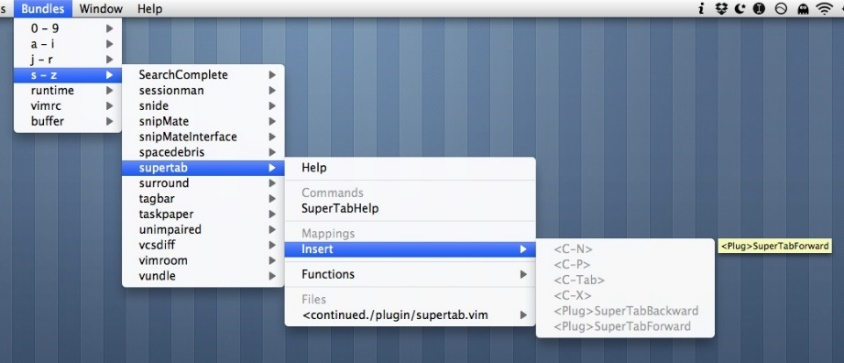
\includegraphics[width=3.7963in,height=1.63208in]{media/media/image3.jpeg}
\caption{GUI Menus Allow Mouse Positional Selection of Software Functionality}
\label{fig:auto:3}
\end{figure}


\section{Chordal Input
Peripherals}\label{chordal-input-peripherals}

Chordsets are peripherals enabling user input commands by actuating
several keys simultaneously (analogous to a piano "chord"). The number
of items selectable for a given number of actuators is the number of
combinations of the individual actuators. For example, there are several
one-hand chordsets (e.g., Figure 5). Given 1 actuator for each finger,
the number of possible selections is 31 - a large enough number to make
simple English text input possible (Seibel, 1962). Chordsets are
sometimes used in contexts (e.g., bicycle handlebars) too small for
standard keyboard.

\begin{figure}[htbp]
\centering
\includegraphics[width=1.16667in,height=1.52621in]{media/media/image4.emf}
\caption{One-handed Chordset}
\label{fig:auto:4}
\end{figure}


The salient feature of chordal input devices is that gestures are
associated with discrete values; for example, a 5-actuator chordset may
associate the 31 possible combinations of actuators with integers in the
range 1-32. Each of these discrete integers can be associated by
software with a distinct software functionality. Examples follow in
future sections.

\section{Device Agnosticism}\label{device-agnosticism}
It is not uncommon for software to allow GUI features designed for one
device to be optionally selected by another device. illustrates a GUI
intended for keyboard selection via number keys allowing positional
selection via mouse click. Another common example is that many software
apps provide \emph{\textbf{keyboard accelerators}} () to associate the
key marks with menu items (Hendy, 2009; Pausch et al., 1991).

\begin{figure}[htbp]
\centering
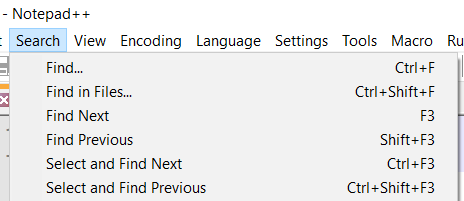
\includegraphics[width=4.83401in,height=2.09404in]{media/media/image5.png}
\caption{Keyboard Accelerators Associate App Commands with Gesture Sequences}
\label{fig:auto:5}
\end{figure}


\emph{\textbf{µLex}} is designed to be \emph{\textbf{device agnostic}} -
\emph{\textbf{µLex}} GUIs present choices that can be selected by any
peripheral with the ability to send key mark, positional, or discrete
numeric information via the OS.

\section{Input Gestures}\label{input-gestures}
It is useful to view the input process in terms of user gestures. As a
trivial example, to input the English lexeme `\textbf{\uline{cat}}` with
a keyboard, keyboards present a \emph{\textbf{choice set}} consisting of
the key marks, users make sequences of three \emph{\textbf{selections}}
from the choice set, and software inputs the lexeme. In general, Lexemes
are input by \emph{\textbf{sequences}} of \emph{\textbf{selections}}
among \emph{\textbf{choice sets}} and \emph{\textbf{selection}} is
completed when \emph{\textbf{actuation}} (press and release) of
\emph{\textbf{actuators}} (keys or mouse buttons) is complete.

For the purposes of this research:

\begin{itemize}
\item
  Keyboard gestures are defined as (re-)positioning the hand and/or
  finger(s) over the keyboard together with \emph{\textbf{actuations}}
  (pressing and releasing) of keys.
\item
  Mouse gestures are defined as (re-)positioning the cursor over GUI
  regions together with actuations of mouse-buttons.
\item
  Chordal gestures are defined as actuating combinations of device
  actuators.
\end{itemize}

\section{Alternative Actuations}\label{alternative-actuations}
Individual marked keys and GUI positional regions can be associated with
several alternative actuations to increase available software
functionalities. Figure 7 illustrates example alternative keyboard
actuations for the `\textbf{B}` key.

\begin{longtable}[]{@{}
  >{\raggedright\arraybackslash}p{(\columnwidth - 2\tabcolsep) * \real{0.3956}}
  >{\raggedright\arraybackslash}p{(\columnwidth - 2\tabcolsep) * \real{0.6044}}@{}}
\toprule
\begin{minipage}[b]{\linewidth}\raggedright
Alternative Actuation
\end{minipage} & \begin{minipage}[b]{\linewidth}\raggedright
Software Functionality
\end{minipage} \\
\midrule
\endhead
B & Insert Lowercase B \\
\textless Shift\textgreater B & Insert Uppercase B \\
\textless Ctrl\textgreater B & Change Selection To/From Boldface \\
\bottomrule
\end{longtable}

Figure Alternative Keyboard
Actuations and Associated Software Functionalities

Once positioned, there are several mouse actuations that software may
associate several different actuations with software functionalities.
Figure 8 enumerates example alternative mouse actuated software
functionalities.

\begin{longtable}[]{@{}
  >{\raggedright\arraybackslash}p{(\columnwidth - 2\tabcolsep) * \real{0.4616}}
  >{\raggedright\arraybackslash}p{(\columnwidth - 2\tabcolsep) * \real{0.5384}}@{}}
\toprule
\begin{minipage}[b]{\linewidth}\raggedright
Alternative Actuation
\end{minipage} & \begin{minipage}[b]{\linewidth}\raggedright
Software Functionality
\end{minipage} \\
\midrule
\endhead
Single Left Click & Move Cursor for Insertion \\
Double Left Click & Select Enclosing Word \\
Triple Left Click & Select Enclosing Paragraph \\
Right Click & Context Menu (Figure 9) \\
\bottomrule
\end{longtable}

Figure Alternative Mouse
Actuations and Associated Software Functionalities

\begin{figure}[htbp]
\centering
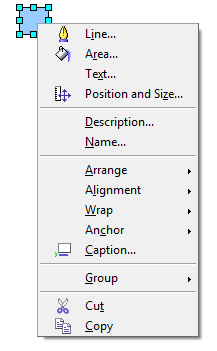
\includegraphics[width=1.0566in,height=1.7102in]{media/media/image6.png}
\caption{Context Menus are Often Displayed as a Result of Clicking Right Mouse Buttons}
\label{fig:auto:6}
\end{figure}


\section{Input Gestures are not Input
Effort}\label{input-gestures-are-not-input-effort}

Gestures and alternative actuations vary in user \emph{\textbf{effort}}:

\begin{itemize}
\item
  Typing `\textbf{1}` requires more effort than `\textbf{a}`.
\item
  Triple click requires more effort than single click.
\item
  Shifting adds effort when capitalizing.
\item
  Three finger chords require more effort than single finger chords.
\end{itemize}

A related set of studies focus on user \emph{\textbf{effort}} for
lexical input. For instance, there are several studies that use
annealing algorithms to discover alternative more
\emph{\textbf{effort-efficient}} keyboard layouts (Francis \& Oxtoby,
2006; Light \& Anderson, 1993; Onsorodi \& Korhan, 2020).

Effort considerations are ignored for the current research, which
attempts to provide a more general measure of \emph{\textbf{gesture}} to
be applied device-agnostically.

Specifically, for this research, each alternative actuation, even if it
involves additional keys, clicks, time, or effort is quantified as a
single gesture.

\section{Gesture/Functionality
Associations}\label{gesturefunctionality-associations}

All GUIs present users with associations of device gestures with
software functionalities. For keyboards, \emph{\textbf{gesture/function
associations}} (\emph{\textbf{GFAs}}) make use of the choices presented
by the \textbf{\uline{marks}} on the individual keys. The marks are used
for character input and - when combined with special keys
\textbf{(\textless ctrl\textgreater{}},
\textbf{\textless alt\textgreater{}},
\textbf{\textless esc\textgreater{}},
\textbf{\textless shift\textgreater{}}) - invoke other functions such as
keyboard accelerators (section 2.5.1, Figure 6).

For mice, touchscreens and other cursor moving devices, GFAs are
positional on the GUI itself (e.g., menus, Figure 8). Many GUIs do
\textbf{\uline{not}} use mice for lexical input. Instead,
\uline{supplemental} software (e.g., virtual keyboards) are used to
provide mouse-click/QWERTY-input GFAs.

\begin{figure}[htbp]
\centering
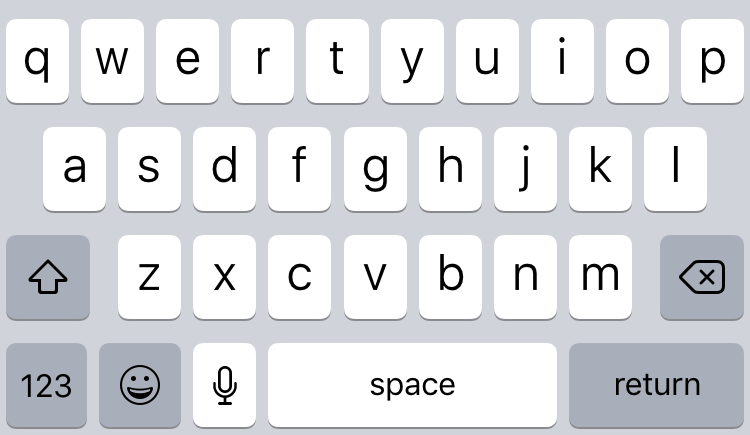
\includegraphics[width=2.78075in,height=1.61111in]{media/media/image7.png}
\caption{Virtual Keyboard for QWERTY Characters}
\label{fig:auto:7}
\end{figure}


For chordsets and other non-marked, non-cursor-positioning devices, GFAs
are provided by supplemental displays (Figure 11), often available only
as images or paper documents.

\begin{figure}[htbp]
\centering
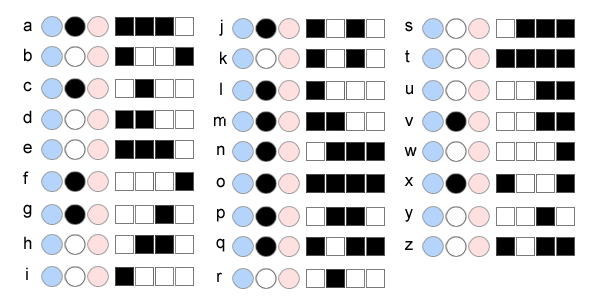
\includegraphics[width=2.87037in,height=1.42881in]{media/media/image8.png}
\caption{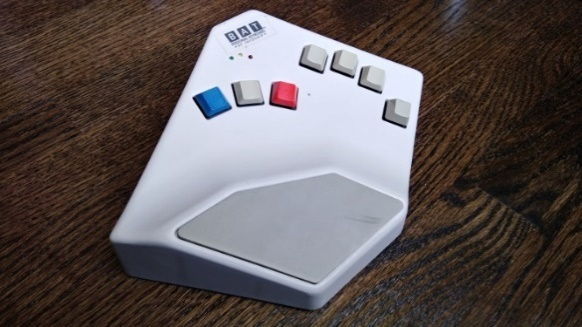
\includegraphics[width=1.43063in,height=1.46296in]{media/media/image9.jpeg}}
\label{fig:auto:8}
\end{figure}


Figure Display for BAT Keyboard
Chord/Letter GFAs

\section{Gestural Efficiency}\label{gestural-efficiency}
By analogy with the definition of \emph{\textbf{efficiency}} from
physics, the basis for analysis of software developed in this research
is \emph{\textbf{Gestural~Efficiency}}~(\emph{\textbf{GE}}):

\[Gestural\ Efficiency\ (GE) = \ \frac{Characters}{Gestures}\]

Where: \emph{\textbf{Gestures}} is the number of distinct user movements
and \emph{\textbf{Characters}} is the number of Unicode characters
input. So, the GE for keyboarding, virtual keyboard clicking, or
chording `\textbf{\uline{cat}}` is:

\[{GE}_{\left\lbrack \text{`cat`} \right\rbrack} = \frac{3\ Characters}{3\ Gestures} = 1\]

The GE for keyboard, virtual keyboard, and basic chordset input of
lexemes is effectively 1 \emph{\textbf{character per gesture}}
(\emph{\textbf{CPG}}):

\[{GE}_{\lbrack Eng,Kbd\rbrack} = \ \frac{1\ Character}{1\ Gesture} = 1\]

Even for single characters, GE is not always 1. For example, one way of
inputting \emph{\textbf{ñ}} with the windows OS is to keyboard the
6‑gesture sequence:

\textbf{\textless Fn\textgreater+\textless NmLk\textgreater{}}\\
\textbf{\textless Alt\textgreater+\textless Num 1\textgreater{}}\\
\textbf{\textless Alt\textgreater+\textless Num 6\textgreater{}}\\
\textbf{\textless Alt\textgreater+\textless Num 4\textgreater{}}\\
\textbf{\textless Fn\textgreater+\textless NmLk\textgreater{}}

Figure 6-Gesture Sequence to
Input \textbf{ñ} on Microsoft Windows

GE for \emph{\textbf{ñ}} using this input method is:

\[{GE}_{\left\lbrack ñ\mathbf{,}kbd \right\rbrack} = \ \frac{1\ Character}{6\ Gestures} = 0.17\]

For some far eastern languages, as Chinese, where users commonly
keyboard 5-12 keyboard gestures to select individual characters
(漢字/\textbf{汉字}, ``hànzì''), such as

\begin{longtable}[]{@{}
  >{\raggedright\arraybackslash}p{(\columnwidth - 4\tabcolsep) * \real{0.3144}}
  >{\raggedright\arraybackslash}p{(\columnwidth - 4\tabcolsep) * \real{0.3353}}
  >{\raggedright\arraybackslash}p{(\columnwidth - 4\tabcolsep) * \real{0.3503}}@{}}
\toprule
\begin{minipage}[b]{\linewidth}\raggedright
\textbf{升} (shēng, ``liter'')
\end{minipage} & \begin{minipage}[b]{\linewidth}\raggedright
\textbf{吊} (diào, ``lift up'')
\end{minipage} & \begin{minipage}[b]{\linewidth}\raggedright
\textbf{闯} (chuăng, ``to rush'')
\end{minipage} \\
\midrule
\endhead
\textbf{迥} (jiǒng, ``distant'') & \textbf{的} (de,
\textbackslash possessive\textbackslash) & \textbf{一} (yī, ``one'') \\
\textbf{是} (shì, ``is'') & \textbf{不} (bù, ``not'') & \textbf{了} (le,
\textbackslash perfective\textbackslash) \\
\bottomrule
\end{longtable}

Figure Sample Simplified Chinese
Characters

The GE for these \textbf{汉字} is:

\[\frac{1\ Character}{12\ Gestures} \leq {GE}_{\lbrack 汉字,kbd\rbrack} \leq \ \frac{1\ Character}{5\ Gestures}\]

Or

\[0.08 \leq {GE}_{\lbrack 汉字,kbd\rbrack} \leq \ 0.20\]

\begin{enumerate}
\def\labelenumi{\arabic{enumi}.}
\setcounter{enumi}{2}
\item
  
\end{enumerate}
